% =====================================================================
%  Distrusting the Radio: Containing Air-Facing Code on Commodity
%  IoT Microcontrollers -- PhD Research Proposal
%  Build: pdflatex proposal && bibtex proposal && pdflatex proposal && pdflatex proposal
%  (or: latexmk -pdf proposal)
% =====================================================================
\documentclass[conference,10pt]{IEEEtran}
\IEEEoverridecommandlockouts

\usepackage[T1]{fontenc}
\usepackage{cite}
\usepackage{amsmath}
\usepackage{graphicx}
\usepackage{xcolor}
\usepackage{microtype}
\usepackage{tikz}
\usetikzlibrary{arrows.meta,positioning,fit,backgrounds,calc}
\usepackage{pgfplots}
\pgfplotsset{compat=1.18}
\usepackage{pgfgantt}
\usepackage{xurl}
\usepackage[hidelinks]{hyperref}

% Placeholders that must be completed before circulation.
\newcommand{\TODO}[1]{\textcolor{red}{[#1]}}
% Code identifiers (underscores printed verbatim).
\newcommand{\sym}[1]{\texttt{\detokenize{#1}}}

\begin{document}

\title{Distrusting the Radio: Containing Air-Facing Code\\on Commodity IoT Microcontrollers\\[0.4em]
{\large PhD Research Proposal}}

\author{\IEEEauthorblockN{Amin Jafarpour}
\IEEEauthorblockA{\textit{School of Computing Science}\\
\textit{Simon Fraser University}\\
Burnaby, BC, Canada\\
\TODO{email address}}
\and
\IEEEauthorblockN{\TODO{Proposed supervisor}}
\IEEEauthorblockA{\textit{\TODO{School or department}}\\
\textit{\TODO{Institution}}\\
\TODO{City, country}\\
\TODO{email address}}}

\maketitle

\begin{abstract}
Wireless microcontrollers such as Espressif's ESP32 family place their most exposed software, the Wi-Fi and Bluetooth stacks that parse attacker-controlled frames, in the same address space as the application, its keys, and the code that can rewrite flash. These stacks ship as precompiled, closed libraries, so developers can neither audit nor patch them, and a single over-the-air memory-safety bug becomes a whole-device compromise; a Bluetooth flaw in this family has already allowed arbitrary code execution from radio range. Two-chip designs, in which an application processor drives a separate radio co-processor over SDIO or SPI, move the stack off the main chip but still trust whatever the co-processor returns. This proposal argues that air-facing code on commodity microcontrollers can be contained, so that its compromise does not imply compromise of the application, its secrets, or its firmware, using only isolation hardware that already ships in these chips and at a cost compatible with radio timing. The work is organized in three thrusts. AirLock-Scope infers the memory, peripheral, interrupt and DMA footprint of closed radio stacks phase by phase, using the chips' own permission hardware as a profiler. AirLock-Cell confines those stacks on single-chip parts by turning the vendor's 128-entry operating-system adapter into a set of gates and by narrowing privileges once initialization ends. AirLock-Link hardens the host of two-chip designs with confined DMA, verified parsers, end-to-end protection, attestation and guaranteed recovery. A preliminary static census of the vendor libraries already shows that, on newer chips, part of the 802.11 stack's mutable state, including a dozen code-pointer slots, lives at fixed addresses reserved by the mask ROM, a constraint that no existing compartmentalization system addresses. Evaluation spans three silicon generations and two instruction-set architectures.
\end{abstract}

\begin{IEEEkeywords}
embedded systems security, compartmentalization, least privilege, wireless protocol stacks, closed binary libraries, network co-processors, ESP32
\end{IEEEkeywords}

% ---------------------------------------------------------------------
\section{Introduction}
\label{sec:intro}

Wireless microcontrollers have become the default substrate of the Internet of Things. A single ESP32-class chip combines one or two application cores, Wi-Fi and Bluetooth radios, and a few hundred kilobytes of SRAM for a few dollars, and the original ESP32 alone has sold more than a billion units~\cite{devreker2024liberating}. On these devices the most exposed software is the radio stack, which we call \emph{air-facing code}: code that parses or acts on input arriving over the air. It processes management frames, link-manager packets and advertisements from anyone within range, usually before any authentication has taken place, and it is large; the three core Wi-Fi libraries for the ESP32-S3 alone define almost two thousand global functions (Section~\ref{sec:prelim}).

It is also the code that developers can least inspect. Espressif's development framework is largely open source, with a notable exception: Wi-Fi, Bluetooth and low-level RF functionality are distributed as precompiled libraries that are linked into the developer's own firmware~\cite{devreker2023unveiling}. Once linked, nothing separates them from the application, its credentials, or the code that can rewrite flash and program eFuses. A memory-safety bug in the radio stack is therefore a whole-device compromise, and such bugs exist. The BrakTooth study found that the Bluetooth Classic implementation in ESP-IDF 4.4 and earlier did not properly restrict the feature page of an incoming LMP Feature Response Extended packet, allowing attackers within radio range to trigger arbitrary code execution on the ESP32~\cite{garbelini2022braktooth,nvd202128139}. In 2019, Espressif issued advisories for three Wi-Fi flaws in its ESP32 and ESP8266 software, chiefly in WPA2-Enterprise support: a zero-PMK installation and two crash bugs~\cite{espressif2019zeropmk}. Protocol-level design flaws such as FragAttacks show that even a faithful implementation of the standard can be vulnerable~\cite{vanhoef2021fragattacks}.

Larger platforms learned to distrust radio firmware the hard way. Remote code execution inside Broadcom Wi-Fi chips was demonstrated and, in Project Zero's work, extended into the host operating system of a phone~\cite{artenstein2017broadpwn,beniamini2017overtheair}, and the coexistence interfaces between Bluetooth and Wi-Fi cores on combination chips enabled inter-chip privilege escalation~\cite{classen2022spectra}. On a microcontroller there is no host operating system to escalate into: the radio stack already runs with the privileges of everything else.

A second architecture is emerging. Espressif's ESP32-P4 has no radio at all; its reference board pairs it with an on-board ESP32-C6 that runs the wireless stacks as a co-processor~\cite{esphostedsdio}, and the host drives it through remote procedure calls over SDIO, SPI or UART~\cite{esphostedmcu}. Thread radio co-processors follow the same pattern over the Spinel protocol~\cite{openthreadcp}. Moving the stack to a second chip changes where the boundary lies but not who is trusted: the host still parses whatever the co-processor sends, and it still sizes its buffers and transfers from values the co-processor supplies. On personal computers, Thunderclap showed that peripherals must be treated as adversaries even behind an IOMMU~\cite{markettos2019thunderclap}; the corresponding discipline is largely absent from microcontroller host drivers.

Existing compartmentalization research does not close this gap. Compiler- and MPU-based systems for microcontrollers~\cite{clements2018aces,kim2018minion,khan2023ec,zhou2022opec,du2022kage,levy2017tock} assume access to the source code being isolated, and most target ARM Cortex-M protection units. Hardware proposals such as UCCA~\cite{tyler2024ucca} and CHERIoT~\cite{amar2023cheriot,amar2025cheriotrtos} can isolate untrusted or closed code but require new silicon. The closed, monolithic radio libraries of Xtensa and RISC-V microcontrollers fall outside all of these assumptions. Meanwhile, the chips themselves ship isolation hardware that mainstream software barely uses. The ESP32-S3 includes a World Controller and a Permission Controller~\cite{esp32s3datasheet}, yet in 2022 Espressif staff reported no stable public code for the former~\cite{espforum2022wcl}; developers who explored the classic ESP32's MMU, MPU and process-ID controller found the documentation lacking and the hardware apparently unused~\cite{espforummmu}; and Espressif's trusted execution environment for its RISC-V parts uses access-permission hardware to protect secure services and keys, not to confine the radio~\cite{esptee}.

This proposal advances the following thesis: \emph{air-facing code on commodity microcontrollers can be contained, so that its compromise does not imply compromise of the application, its secrets, or its firmware, using only isolation hardware that already ships in these chips, at a cost compatible with radio timing.} We call the resulting framework AirLock and organize the work in three thrusts, summarized in Fig.~\ref{fig:arch}. AirLock-Scope infers what closed radio stacks actually touch, phase by phase. AirLock-Cell confines them on single-chip parts. AirLock-Link hardens the host of two-chip designs against a fully compromised co-processor. The planned contributions are a cross-generation characterization and public dataset of closed radio-stack footprints; a containment monitor for single-chip parts that narrows privileges after initialization; a hardened host interface with confined DMA, verified parsers, attestation and guaranteed recovery; and an analysis of which guarantees each hardware generation can and cannot provide, together with the minimal hardware changes that would close the gaps. All three thrusts are evaluated on the classic ESP32 (Xtensa LX6), the ESP32-S3 (Xtensa LX7) and the ESP32-P4 with its ESP32-C6 co-processor (RISC-V).

The work is timely beyond its research interest. The EU Cyber Resilience Act requires products with digital elements to be designed, developed and produced to limit attack surfaces, including external interfaces, and to reduce the impact of incidents through appropriate exploitation-mitigation mechanisms~\cite{cra2024}, and its essential requirements apply from December 2027. Radio containment is a direct and testable response to both requirements for the cheapest connected devices on the market.

The rest of this proposal reviews the relevant software and hardware (Section~\ref{sec:background}), reports a preliminary static census of the vendor libraries (Section~\ref{sec:prelim}), defines the threat model (Section~\ref{sec:threat}) and research questions (Section~\ref{sec:rq}), describes the three thrusts (Section~\ref{sec:approach}) and their evaluation (Section~\ref{sec:eval}), situates the work (Section~\ref{sec:related}), and closes with the timeline, risks and ethical considerations.

% ---------------------------------------------------------------------
\begin{figure*}[t]
\centering
\resizebox{\textwidth}{!}{%
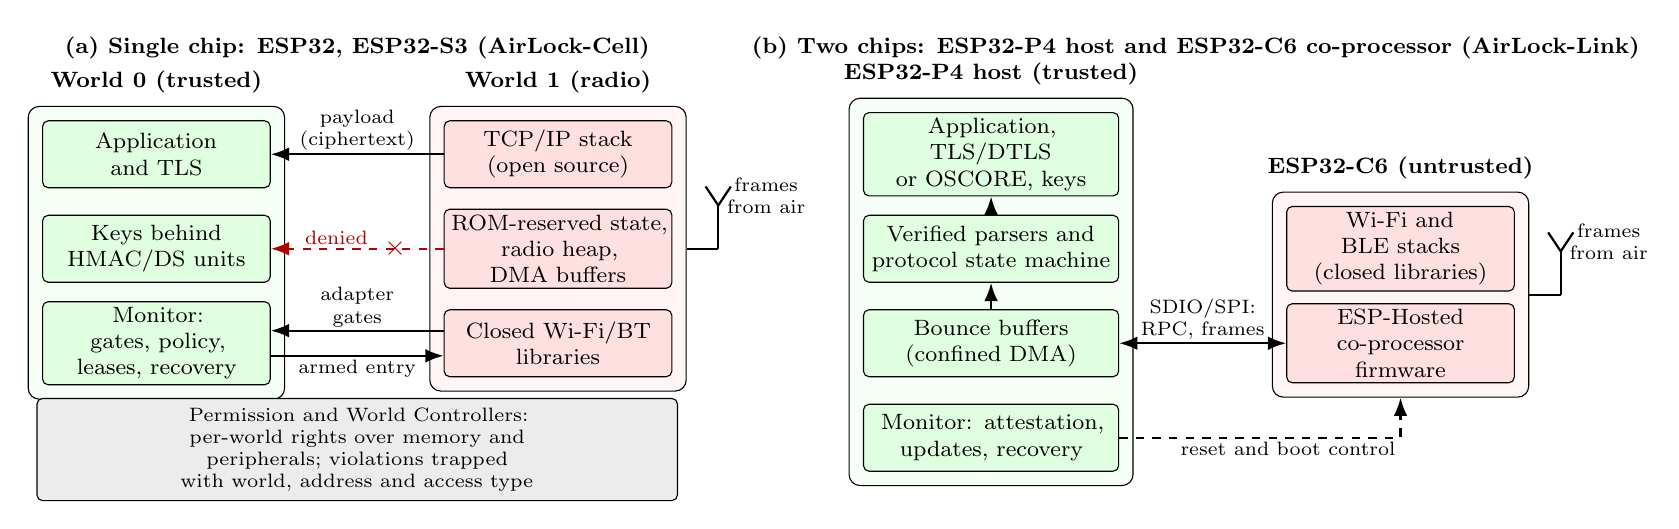
\begin{tikzpicture}[font=\footnotesize, >=Latex,
  cell/.style={draw, rounded corners=2pt, align=center, minimum height=0.85cm, text width=2.75cm, inner sep=2pt},
  tr/.style={cell, fill=green!12},
  ut/.style={cell, fill=red!12},
  lbl/.style={font=\scriptsize, align=center, inner sep=1pt},
]
% ----------------------------- panel (a)
\node[tr] (a-app)  at (0,0)     {Application\\and TLS};
\node[tr] (a-keys) at (0,-1.2)  {Keys behind\\HMAC/DS units};
\node[tr] (a-mon)  at (0,-2.4)  {Monitor: gates, policy,\\leases, recovery};
\node[ut] (a-tcp)  at (5.1,0)   {TCP/IP stack\\(open source)};
\node[ut] (a-rom)  at (5.1,-1.2){ROM-reserved state,\\radio heap, DMA buffers};
\node[ut] (a-lib)  at (5.1,-2.4){Closed Wi-Fi/BT\\libraries};
\begin{scope}[on background layer]
  \node[draw, rounded corners, fill=green!4, fit=(a-app)(a-mon), inner sep=5pt] (a-w0) {};
  \node[draw, rounded corners, fill=red!4,   fit=(a-tcp)(a-lib), inner sep=5pt] (a-w1) {};
\end{scope}
\node[font=\footnotesize\bfseries, above=1pt of a-w0] {World 0 (trusted)};
\node[font=\footnotesize\bfseries, above=1pt of a-w1] {World 1 (radio)};
\draw[->, thick] (a-tcp.west) -- node[lbl, above] {payload\\(ciphertext)} (a-app.east);
\draw[->, thick, dashed, red!70!black] (a-rom.west) -- node[lbl, above, pos=0.62] {denied} node[pos=0.28, font=\normalsize, red!70!black] {$\times$} (a-keys.east);
\draw[->, thick] ([yshift=1.6mm]a-lib.west) -- node[lbl, above] {adapter\\gates} ([yshift=1.6mm]a-mon.east);
\draw[->, thick] ([yshift=-1.6mm]a-mon.east) -- node[lbl, below] {armed entry} ([yshift=-1.6mm]a-lib.west);
\node[draw, fill=gray!15, rounded corners=2pt, minimum height=0.7cm, text width=7.9cm, align=center, font=\scriptsize] (a-hw) at (2.55,-3.75)
  {Permission and World Controllers: per-world rights over memory and\\peripherals; violations trapped with world, address and access type};
\draw[thick] (a-w1.east) -- ++(0.4,0) coordinate (a-ant);
\draw[thick] (a-ant) -- ++(0,0.55) coordinate (a-top);
\draw[thick] (a-top) -- ++(-0.16,0.24);
\draw[thick] (a-top) -- ++(0.16,0.24);
\node[lbl, anchor=west] at ([xshift=2pt,yshift=0.12cm]a-top) {frames\\from air};
\node[font=\footnotesize\bfseries] at (2.55,1.35) {(a) Single chip: ESP32, ESP32-S3 (AirLock-Cell)};
% ----------------------------- panel (b)
\node[tr, text width=3.1cm] (b-app)   at (10.6,0)     {Application, TLS/DTLS\\or OSCORE, keys};
\node[tr, text width=3.1cm] (b-parse) at (10.6,-1.2)  {Verified parsers and\\protocol state machine};
\node[tr, text width=3.1cm] (b-buf)   at (10.6,-2.4)  {Bounce buffers\\(confined DMA)};
\node[tr, text width=3.1cm] (b-mon)   at (10.6,-3.6)  {Monitor: attestation,\\updates, recovery};
\node[ut] (b-stack) at (15.8,-1.2) {Wi-Fi and BLE stacks\\(closed libraries)};
\node[ut] (b-fw)    at (15.8,-2.4) {ESP-Hosted\\co-processor firmware};
\begin{scope}[on background layer]
  \node[draw, rounded corners, fill=green!4, fit=(b-app)(b-mon), inner sep=5pt] (b-host) {};
  \node[draw, rounded corners, fill=red!4,   fit=(b-stack)(b-fw), inner sep=5pt] (b-cp) {};
\end{scope}
\node[font=\footnotesize\bfseries, above=1pt of b-host] {ESP32-P4 host (trusted)};
\node[font=\footnotesize\bfseries, above=1pt of b-cp] {ESP32-C6 (untrusted)};
\draw[<->, thick] (b-fw.west) -- node[lbl, above] {SDIO/SPI:\\RPC, frames} (b-buf.east);
\draw[->, thick] (b-buf.north) -- (b-parse.south);
\draw[->, thick] (b-parse.north) -- (b-app.south);
\draw[->, thick, dashed] (b-mon.east) -| node[lbl, pos=0.3, below] {reset and boot control} (b-cp.south);
\draw[thick] (b-cp.east) -- ++(0.4,0) coordinate (b-ant);
\draw[thick] (b-ant) -- ++(0,0.55) coordinate (b-top);
\draw[thick] (b-top) -- ++(-0.16,0.24);
\draw[thick] (b-top) -- ++(0.16,0.24);
\node[lbl, anchor=west] at ([xshift=2pt,yshift=0.12cm]b-top) {frames\\from air};
\node[font=\footnotesize\bfseries] at (13.2,1.35) {(b) Two chips: ESP32-P4 host and ESP32-C6 co-processor (AirLock-Link)};
\end{tikzpicture}}
\caption{AirLock overview. (a) On single-chip parts, the closed radio libraries, the TCP/IP stack and the radio's ROM-reserved state run in the untrusted world; their calls through the vendor's operating-system adapter become gates into a small monitor, and only transport payload crosses into the trusted world. (b) In two-chip designs the host treats the co-processor as untrusted: transfers land only in confined bounce buffers, are decoded by verified parsers, and application data crosses the link only as ciphertext; where the board wires them, the host keeps control of the co-processor's reset and boot lines.}
\label{fig:arch}
\end{figure*}

% ---------------------------------------------------------------------
\section{Background}
\label{sec:background}

\subsection{Radio Software on ESP32-Class Microcontrollers}

For each chip, Espressif publishes the Wi-Fi stack as a set of static archives: three core libraries (\sym{libcore}, \sym{libnet80211} and \sym{libpp}) and optional ones for ESP-NOW, mesh networking, SmartConfig and WAPI~\cite{esp32wifilib}. PHY calibration, coexistence arbitration and the Bluetooth controller ship as further closed libraries. The archives are written against an operating-system adapter rather than against FreeRTOS directly. In the ESP-IDF master branch as of November 2026, the adapter structure \sym{wifi_osi_funcs_t} (adapter version~9) declares 128 function pointers~\cite{espidfosadapter}. They cover interrupt allocation and masking; semaphores, mutexes, queues and event groups; task creation and pinning; general and internal-RAM memory allocation; twelve non-volatile storage (NVS) operations; PHY and clock control; timers; random numbers; logging; and 24 coexistence hooks. The adapter is a stable seam. The Rust \sym{esp-wifi} project reimplements it for each chip in order to run the same closed libraries under a different runtime~\cite{espwifirust}.

The adapter is not the only seam, however. Section~\ref{sec:prelim} shows that the libraries also reference ROM routines, other closed libraries, ESP-IDF data and a handful of C-library functions directly. Their resource needs also change over time: engineers building an open Wi-Fi MAC for the classic ESP32 logged 53,286 peripheral accesses during Wi-Fi initialization, whereas sending a packet takes about ten calls~\cite{hackaday2024openmac}. That project, which aims at a Wi-Fi-capable, blob-free SDK for the ESP32~\cite{openmacrepo}, and a derived open ESP32-C3 driver built for static worst-case energy analysis~\cite{mudraje2025opendrivers} document much of the hardware's behavior and give this work a source of ground truth.

\subsection{Isolation Hardware Across Three Generations}

The classic ESP32 (dual-core Xtensa LX6) provides memory-management and memory-protection units and an asymmetric process-ID (PID) controller~\cite{esp32trm}. Developers who tried to build isolated applications with them report incomplete documentation of the MMU and MPU~\cite{espforummmu}, and Espressif's own proof of concept for privilege separation on this chip ran into limitations that led the company to design dedicated isolation peripherals for later parts~\cite{parekhprivsep}.

Those peripherals appear on the ESP32-S3 (dual-core Xtensa LX7) as a Permission Controller and a World Controller~\cite{esp32s3datasheet}. Espressif documents their semantics for the ESP32-C3, where they were introduced~\cite{espprivsepwcl}. Execution happens in one of two worlds. Software arms a trigger address, and the World Controller switches the CPU from World~0 (secure) to World~1 (non-secure) when that address is fetched; any interrupt or exception switches it back to World~0. Every memory or peripheral access carries the world of its requester, and the Permission Controller holds an independently configured permission set per world covering internal and external memory and all peripherals. On a violation it can raise an interrupt that records the violating world, the address and the attempted access (read, write or execute). The S3's register map exposes per-core status registers for world-switch entries~\cite{esp32s3pac}. ESP-IDF uses permission hardware on these chips for single-world memory protection, but we are not aware of a maintained component that runs code in the second world on the S3.

The ESP32-P4 (a dual-core RISC-V high-performance system plus a low-power RISC-V core) lists TEE, access-permission management (APM) and PMP/PMA blocks alongside a Key Manager in its datasheet~\cite{esp32p4datasheet}. On the ESP32-C6, where Espressif documents the equivalent blocks in detail, its TEE framework runs in machine mode and the application in user mode; a TEE controller assigns a security mode to each bus master, including DMA, and APM grants each mode permissions over address ranges, covering masters that PMP and PMA cannot govern, such as the low-power core and the general-purpose DMA engine~\cite{esptee}. Espressif's product-security documentation lists TEE support for the C6, with the H2 in preview and the C5 and C61 planned, and does not list the P4~\cite{espsecframeworks}. Across generations, key-holding peripherals give the trusted side a way to keep secrets out of reach even of software that runs with its privileges: HMAC and digital-signature units on the S3, and on the P4 a Key Manager whose keys are bound to a per-chip hardware unique key and never exposed to software-accessible memory~\cite{esp32p4security}.

\subsection{Two-Chip Designs}

ESP-Hosted-MCU turns Espressif chips into communication co-processors: the host sends RPC commands over SPI, SDIO or UART, the co-processor executes them, and the implementation builds on ESP-IDF, \sym{esp_wifi_remote} and \sym{protobuf-c}~\cite{esphostedmcu}. On the P4 reference board, the host brings up Wi-Fi through the on-board ESP32-C6 on SDMMC slot~1~\cite{esphostedsdio}, and the host can push new co-processor firmware through a begin, write, end and activate sequence of RPCs~\cite{esphostedota}. OpenThread's radio co-processor design is analogous: the core of the Thread stack lives on the host, and a minimal MAC controller runs on the radio device, connected over a serial link that speaks Spinel~\cite{openthreadcp}. In each case the host-side transport driver and message decoder form the trust boundary that matters, and, to our knowledge, they are written assuming a well-behaved co-processor.

% ---------------------------------------------------------------------
\section{Preliminary Evidence: A Static Census}
\label{sec:prelim}

To ground the research questions, we performed a static census of the closed Wi-Fi libraries for three chips: the classic ESP32, the ESP32-S3, and the ESP32-C6, which is both the co-processor on P4 boards and the RISC-V counterpart of the S3. We parsed the archives at the \sym{esp32-wifi-lib} revision pinned by ESP-IDF master in November 2026 (commit \sym{07e8d01})~\cite{esp32wifilib} with standard ELF tools, collected every global symbol that each library defines or references, and resolved the references against the other radio libraries and against each chip's mask-ROM linker scripts in ESP-IDF~\cite{espidfosadapter}. ROM-resolved symbols were then classified by address as ROM-resident routines and constant tables, or as variables at fixed addresses in RAM reserved by the ROM.

The three core libraries comprise 81 object files with 363\,kB of executable sections on the classic ESP32, 81 files with 303\,kB on the S3, and 105 files with 416\,kB on the C6, defining 1,977, 1,996 and 2,497 global functions respectively. These are pre-link sizes and thus upper bounds on what a given application links. On all three chips the libraries reach the operating-system adapter through a single pointer symbol, \sym{g_osi_funcs_p}. Beyond the adapter and the libraries themselves, they reference 73, 149 and 204 external symbols (Fig.~\ref{fig:census}).

The breakdown differs sharply between generations. On the classic ESP32, all 27 ROM-resolved references are C-library, compiler-runtime or ROM utility routines, and none resolves into ROM-reserved RAM. On the S3, 54 of the 86 ROM-resolved references are variables at fixed addresses in ROM-reserved RAM; on the C6, 76 of 142 are. On both newer chips, twelve of these fixed-address variables have names indicating function pointers or function tables, among them the adapter pointer itself, the tables \sym{net80211_funcs} and \sym{pp_wdev_funcs}, and callbacks such as \sym{sta_rxcb} and \sym{g_tx_done_cb_func}. The remaining 46, 63 and 62 references go to PHY-library entry points, ESP-IDF event and regulatory data, and a few C-library functions called directly rather than through the adapter, such as \sym{free} and \sym{sprintf} on the S3.

Three implications shape the proposed work. First, the adapter is the dominant but not the only boundary, so every direct reference must be resolved either into the radio compartment or into a gate. Second, on newer chips part of the stack's mutable state is pinned by the mask ROM at fixed addresses, so the compartment layout must carve those addresses out of ROM-reserved memory, and the granularity of the permission hardware decides whether that is possible without over-granting. Third, because a dozen of these slots hold code pointers that the radio compartment can overwrite, trusted code must never call through them; a containment design has to treat every such slot as attacker-controlled. The census is static and symbol-level. It says nothing about memory-mapped I/O, DMA or run-time behavior, which is what Thrust~1 adds.

\begin{figure}[t]
\centering
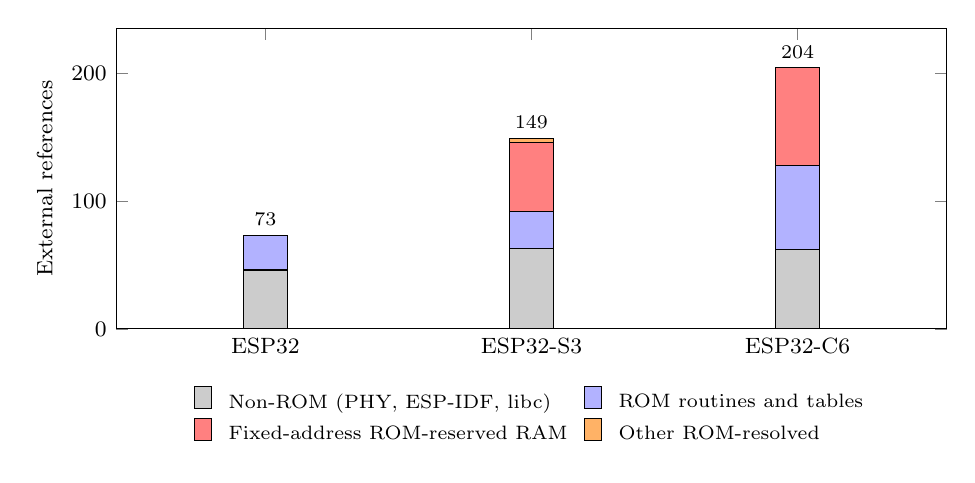
\begin{tikzpicture}
\begin{axis}[
  ybar stacked,
  bar width=16pt,
  width=\columnwidth,
  height=5.4cm,
  ymin=0, ymax=235,
  ylabel={External references},
  ylabel style={font=\footnotesize},
  symbolic x coords={ESP32,ESP32-S3,ESP32-C6},
  xtick=data,
  enlarge x limits=0.28,
  tick label style={font=\footnotesize},
  legend style={font=\scriptsize, at={(0.5,-0.17)}, anchor=north, legend columns=2, draw=none, column sep=4pt},
  legend cell align=left,
]
\addplot+[fill=gray!40, draw=black] coordinates {(ESP32,46) (ESP32-S3,63) (ESP32-C6,62)};
\addplot+[fill=blue!30, draw=black] coordinates {(ESP32,27) (ESP32-S3,29) (ESP32-C6,66)};
\addplot+[fill=red!50, draw=black] coordinates {(ESP32,0) (ESP32-S3,54) (ESP32-C6,76)};
\addplot+[fill=orange!60, draw=black] coordinates {(ESP32,0) (ESP32-S3,3) (ESP32-C6,0)};
\legend{{Non-ROM (PHY, ESP-IDF, libc)}, {ROM routines and tables}, {Fixed-address ROM-reserved RAM}, {Other ROM-resolved}}
\node[above, font=\scriptsize] at (axis cs:ESP32,73) {73};
\node[above, font=\scriptsize] at (axis cs:ESP32-S3,149) {149};
\node[above, font=\scriptsize] at (axis cs:ESP32-C6,204) {204};
\end{axis}
\end{tikzpicture}
\caption{External references of the core Wi-Fi libraries (\sym{libcore}, \sym{libnet80211}, \sym{libpp}) beyond the libraries themselves, by how they resolve. Static census at \sym{esp32-wifi-lib} commit \sym{07e8d01} and ESP-IDF master, November 2026.}
\label{fig:census}
\end{figure}

% ---------------------------------------------------------------------
\section{Threat Model and Security Goals}
\label{sec:threat}

The adversary is remote. It is within radio range of the device, or controls a network or peer that the device communicates with, and it can transmit arbitrary frames at any time. We assume it can exploit a memory-safety or logic bug in air-facing code and thereby execute arbitrary code with that code's privileges: inside the radio compartment on single-chip parts, and anywhere on the co-processor in two-chip designs. We make no assumption about intent inside that boundary, so the same guarantees cover a closed library that is merely buggy and one that has been tampered with in the supply chain. Having gained a foothold, the adversary aims to take over the application, to read secrets or misuse the peripherals that hold them, to persist by rewriting flash, burning eFuses or changing boot configuration, to brick the device, to falsify sensing or actuation, or to starve the rest of the system.

We trust the isolation hardware to behave as documented or as we characterize it, the boot ROM, correctly configured secure boot and flash encryption, and a small monitor together with the application code it protects. Physical attacks, including invasive probing, fault injection and side channels, are out of scope, as are jamming, weaknesses in the 802.11 and Bluetooth protocols themselves, and vulnerabilities in the trusted application; containment nevertheless limits the damage that several of these can cause.

Against this adversary the framework pursues five goals. \textbf{G1 (integrity):} compromised air-facing code cannot modify code or data outside its compartment. \textbf{G2 (secrecy):} it cannot read key material and can invoke key-holding peripherals only through mediated services. \textbf{G3 (persistence):} it cannot write to the flash or eFuse controllers, change boot configuration, or alter the isolation configuration once that configuration is locked. \textbf{G4 (bounded impact and recovery):} it can deny network service but cannot starve trusted tasks beyond a configured budget, and the monitor can quarantine and restart it without rebooting the application; in two-chip designs, the host can always reset and reprovision the co-processor. \textbf{G5 (boundary integrity):} a compromised co-processor cannot cause host writes outside designated buffers, cannot induce memory errors in host-side parsing, cannot pass off modified firmware as authentic after a reset, and observes application data only as ciphertext. We do not attempt to protect data that the radio must handle in plaintext, such as Wi-Fi credentials and link-layer metadata, nor do we guarantee network availability. Applications that send plaintext over the network gain no confidentiality from containment; they gain the integrity of everything else on the device.

% ---------------------------------------------------------------------
\section{Research Questions}
\label{sec:rq}

\textbf{RQ1 (footprint).} Which memory regions, peripherals, interrupts, DMA engines and ROM-reserved state do closed radio stacks require; how do these requirements vary across lifecycle phases and chip generations; and how precisely can they be inferred without source code?

\textbf{RQ2 (single-chip containment).} Can the isolation hardware already present in commodity microcontrollers confine closed radio stacks to their inferred footprint without violating radio timing, at what cost, and which of G1 to G4 does each generation support?

\textbf{RQ3 (two-chip boundary).} What must a host enforce to remain secure against a fully compromised network co-processor, and can it do so within the bandwidth, latency and energy budgets of SDIO and SPI links?

\textbf{RQ4 (limits).} Which goals are unattainable on each generation, why, and what minimal hardware features would make them attainable?

% ---------------------------------------------------------------------
\section{Approach}
\label{sec:approach}

The three thrusts share one pipeline: Scope produces the policies that Cell and Link enforce, and the results of enforcement feed back into Scope as observed violations.

\subsection{Thrust 1: AirLock-Scope, Footprint Inference}

Scope combines static and dynamic evidence into a phase-annotated \emph{radio capability manifest} for each chip and library version. The static stage extends the census of Section~\ref{sec:prelim} into a dependency graph spanning the radio libraries, the ROM and ESP-IDF, and it recovers constant peripheral addresses from the binaries. This is tractable because Xtensa code loads 32-bit constants from literal pools and RISC-V code materializes them with short, recognizable instruction sequences.

The dynamic stage uses the isolation hardware itself as a profiler. Scope places the radio code in the unprivileged world with a deliberately small permission set and runs the permission hardware in a learning mode analogous to the permissive mode of SELinux: each violation is recorded with its world, address and access type, the containing region is granted, and execution resumes. Because each region traps once rather than each access, even the tens of thousands of peripheral accesses of initialization cost a bounded number of traps. Every adapter call is logged with its arguments and call site, and lifecycle events (initialization, calibration, scanning, association, steady state, power save, coexistence arbitration and teardown) partition the trace into phases. JTAG debugging through the ESP-Prog adapters and the P4's built-in USB-JTAG interface~\cite{espprog2,esp32p4jtag} confirms specific observations, for example writes to the code-pointer slots that the census identified.

A scenario suite that exercises station and access-point modes, WPA2, WPA3 and enterprise authentication, ESP-NOW, Bluetooth and coexistence drives coverage. Paths that are never observed are an inherent limitation of dynamic analysis, so each manifest carries a default action for unobserved accesses: trap-and-log during research, deny-and-recover in deployment. Manifests are regenerated automatically for every ESP-IDF release, which turns drift between library versions into a measured quantity rather than a silent failure, and the reverse-engineered documentation of the open-MAC project~\cite{openmacrepo,devreker2024liberating} serves as ground truth for register semantics.

\subsection{Thrust 2: AirLock-Cell, Single-Chip Containment}

Cell partitions a single-chip device into a trusted world, which holds the application, TLS, keys and a small monitor, and a radio world, which holds the closed libraries, their private heap, the ROM-reserved state identified by Scope, and the open TCP/IP stack. Placing the TCP/IP stack with the radio is deliberate: all parsing of attacker-controlled packets then happens in the untrusted world, and what crosses into the trusted world is reassembled transport payload, which for TLS-protected applications is ciphertext that the trusted TLS stack authenticates. The application reaches the network stack through a narrow socket interface implemented as calls into the radio world, and every value returned is treated as tainted, in the manner of RLBox~\cite{narayan2020rlbox}. Following the structure of Espressif's privilege-separation framework, in which a protected application owns the kernel and a user application runs in the non-secure world~\cite{parekhprivsep}, the RTOS kernel stays in the trusted world and radio tasks run as unprivileged tasks whose resumption the scheduler arms into the radio world.

Calls from the radio libraries into the operating system become gates. Each of the 128 adapter entries points to a stub that enters the trusted world through a deliberate exception (\sym{SYSCALL} on Xtensa, \sym{ECALL} on RISC-V), which the hardware already routes to the trusted side, and the monitor validates every argument before acting. Operating-system objects are exposed to the radio as opaque handles rather than as pointers into trusted memory; memory allocation is served from a radio-private heap; and storage operations are confined to the radio's own NVS namespace, which still lets the Wi-Fi library persist its configuration. The direct references found by the census are either relocated into the radio world, as with the C-library helpers, or redirected to gates. ROM routines execute in place for both worlds; because each access is checked against the permissions of the calling world~\cite{espprivsepwcl}, ROM code called from the radio world cannot reach trusted memory, but stateful ROM routines whose state lives in shared ROM-reserved RAM must not be used by the trusted world, a constraint that Scope's dependency graph makes checkable.

Two hardware questions are decisive. The first is interrupts. Because any interrupt returns the CPU to the secure world~\cite{espprivsepwcl}, a radio interrupt costs a switch into the monitor, a switch into the radio's handler, and a return, and at high packet rates this path could threaten throughput. Cell will measure it, keep handlers short, batch notifications, and evaluate routing selected interrupts to the radio world permanently where the hardware allows it. The second is DMA. The radio's own DMA engines write received frames into memory using descriptors that the radio code programs. If the permission hardware does not constrain those engines as bus masters, a compromised radio could aim them at trusted memory and defeat G1 regardless of how the CPU is confined. On the C6, Espressif's documentation shows APM governing DMA masters~\cite{esptee}; for the S3's radio DMA the question is open, and we will settle it experimentally early in the project because the answer determines which goals the S3 can meet. The classic ESP32's reference manual describes MPU tables for DMA and peripherals~\cite{esp32trm}, which we will characterize in the same way.

Cell enforces \emph{temporal least privilege}. The manifest's initialization phase grants the broad register access that calibration requires; once initialization completes, the monitor revokes it and leaves only the steady-state set, re-granting narrow, time-bounded leases for events such as channel changes or recalibration. Where the hardware provides lock bits, the steady-state configuration is locked. Because errors in hand-written permission configurations are easy to make and hard to see, Cell encodes each generated configuration and the security invariants (no radio-world write to trusted memory or to the flash, eFuse or permission registers, and no trusted-world execution from radio-writable memory) as SMT constraints and checks them on every build.

When the permission hardware reports a violation, the monitor quarantines the radio world by masking its interrupts and suspending its tasks, resets the radio peripherals, and reinitializes the stack from the trusted side while preserving application state; repeated violations escalate to a full reboot. Cell targets the S3 first. On the classic ESP32, whose isolation hardware is less capable and less documented, we will establish which subset of G1 to G4 is achievable, and that partial result is itself an answer to RQ4. If the C6 on the P4 boards can be used standalone, it offers a RISC-V single-chip counterpart in which the monitor runs in machine mode and the radio in user mode, using PMP and APM as Espressif's TEE does~\cite{esptee}.

\subsection{Thrust 3: AirLock-Link, Distrusting the Co-Processor}

Link begins by enumerating the host-side attack surface of ESP-Hosted-MCU on the P4: transport headers with their lengths and offsets, protobuf-encoded RPC responses and events, data frames passed to the network stack, and every place where a value supplied by the co-processor influences a buffer size, a copy length or a subsequent transfer. Unlike a PCIe device, an SDIO or SPI co-processor cannot choose the host addresses at which its data lands, because the host's controller writes into buffers that the host driver describes. The danger lies instead in what the host does with the lengths, offsets and contents it receives, and Link hardens the host in five layers.

\emph{Transport confinement} restricts the host's SDIO and SPI DMA to a pool of bounce buffers and never uses a co-processor-supplied length or offset as a pointer, so that even a bug in the host driver cannot direct a transfer outside the pool. Whether the P4's APM can enforce this on its SDMMC and SPI controllers, as the C6's APM does for its DMA masters~\cite{esptee}, is an open question we will answer experimentally, falling back to driver-enforced checks and guard regions if it cannot. \emph{Verified parsing} replaces hand-written decoders for transport headers and RPC messages with parsers generated from a format specification by EverParse, which proves memory safety and functional correctness~\cite{ramananandro2019everparse,swamy2022everparse3d}, or with memory-safe Rust code where a specification is impractical. This follows the language-theoretic security principle that input handling should be a recognizer for a precisely specified language~\cite{sassaman2011halting}. A \emph{protocol state machine} on the host accepts only responses to outstanding requests, bounds unsolicited events by rate and memory, and sanity-checks semantic values. \emph{End-to-end protection} terminates TLS, DTLS or OSCORE on the host, so that the co-processor carries only ciphertext of application data and never holds long-term application secrets.

The fifth layer is \emph{identity and recovery}. Drawing on SPDM's model of device authentication and firmware measurement~\cite{dmtf2023spdm}, the host challenges the co-processor after every reset for evidence of the firmware it booted. Espressif's TEE, which the C6 supports~\cite{espsecframeworks}, already offers an attestation service that issues ECDSA-signed tokens~\cite{espteeguide}; Link would relay such tokens over the RPC channel and verify them on the host. The host already pushes co-processor firmware through the existing RPC update sequence~\cite{esphostedota}; Link authenticates those updates end to end and keeps a known-good image. If the host also controls the co-processor's reset line, it can guarantee recovery within a time bound, the property that Lazarus provides with a TEE on a single chip~\cite{huber2020lazarus}.

Link is evaluated against an adversarial co-processor. Because ESP-Hosted supports the classic ESP32 and the S3 as co-processors as well as the C6~\cite{esphostedsdio}, spare boards can run firmware that speaks the ESP-Hosted transport but emits malformed headers, inconsistent lengths, unsolicited RPCs and floods. The same methodology transfers to Spinel-based Thread radio co-processors~\cite{openthreadcp}, which we will analyze as a generalization study.

% ---------------------------------------------------------------------
\section{Evaluation Plan}
\label{sec:eval}

The testbed comprises classic ESP32 boards \TODO{record silicon revision}, ESP32-S3 boards, and ESP32-P4 boards of revision v3.x with on-board ESP32-C6 co-processors, together with an ESP-Prog and an ESP-Prog-2 debug adapter. The ESP-Prog-2 bridges JTAG for the ESP32, S2, S3 and C3~\cite{espprog2}, while the P4 is debugged through its built-in USB-JTAG interface~\cite{esp32p4jtag}. Radio experiments run inside an RF-shielded enclosure against a dedicated access point, and energy is measured with a shunt-based power monitor on each board's supply.

Security is evaluated in four ways. \emph{Compromise emulation} instruments a test build to run attacker-controlled code inside the radio compartment, which then attempts every post-compromise action in the threat model: writing trusted code and data, reading key material or invoking the HMAC, digital-signature, ECDSA and Key Manager peripherals, programming the flash and eFuse controllers, reconfiguring the isolation hardware, aiming DMA at trusted memory, corrupting code-pointer slots that trusted code might call, and monopolizing the CPU or interrupts. For each chip we report, goal by goal, which actions are blocked, which are detected and recovered from, and which succeed. \emph{CVE-informed capability models} use publicly documented ESP32 radio vulnerabilities, including the BrakTooth code-execution flaw~\cite{nvd202128139} and the 2019 Wi-Fi flaws~\cite{espressif2019zeropmk}, to parameterize realistic post-exploitation capabilities without reproducing any exploit. \emph{Boundary testing} runs the adversarial co-processor, together with coverage-guided fuzzing of the host's transport and RPC decoders compiled with sanitizers on a workstation, before and after hardening. \emph{Formal checks} cover the SMT invariants of every generated configuration and the EverParse proofs, and we report the size of the trusted computing base in lines of code.

Performance is measured against unmodified ESP-IDF: TCP and UDP throughput, round-trip latency and jitter, association and address-acquisition time, missed Bluetooth connection events, coexistence behavior, cycles per world switch and per gate, interrupt latency, RAM and flash overhead, and energy per megabyte and in power-save mode. Our target is a throughput reduction below ten percent with no additional missed connection events at nominal load; if that proves unattainable, we will characterize the trade-off between privilege granularity and overhead instead. Compatibility is measured by running unmodified ESP-IDF example applications (station, access point, provisioning, a BLE GATT server and ESP-NOW) and counting the source changes they require, with a target of none at the application level.

Three workloads represent deployments: an MQTT-over-TLS sensor node, an over-the-air update client, and a cyber-physical controller in which the device acts as a remote terminal unit for the C-Town water-distribution benchmark~\cite{taormina2018batadal}, simulated in WNTR~\cite{klise2017wntr} with the hardware in the loop, so that the effect of isolation on control deadlines is measured directly. Baselines are unmodified ESP-IDF; Espressif's TEE on the C6, which protects keys but leaves the radio unconfined~\cite{esptee}; and, for context, the published overheads of microcontroller compartmentalization systems~\cite{clements2018aces,khan2023ec}.

% ---------------------------------------------------------------------
\section{Related Work}
\label{sec:related}

\emph{Microcontroller compartmentalization.} ACES automatically derives compartments for bare-metal firmware and enforces them with the ARMv7-M MPU~\cite{clements2018aces}. MINION switches customized memory views for real-time systems~\cite{kim2018minion}. EC compartmentalizes RTOS kernels and bare-metal firmware through intra-kernel isolation and motivates the problem with a drone taken over through a compromised Wi-Fi system-on-chip~\cite{khan2023ec}. OPEC isolates operations in bare-metal firmware~\cite{zhou2022opec}, Kage protects control flow on real-time systems~\cite{du2022kage}, and Tock isolates processes with memory-protection hardware under a kernel written in Rust~\cite{levy2017tock}. These systems rely on source code or a compiler pass over the code being isolated, and most target ARM Cortex-M protection hardware; none confines a closed, monolithic vendor radio library, and none targets Xtensa.

\emph{Hardware for untrusted code.} UCCA is a formally verified hardware architecture that isolates untrusted code sections, including closed third-party libraries, prototyped on an open MSP430 core~\cite{tyler2024ucca}. CHERIoT co-designs a capability instruction set and an RTOS for fine-grained, memory-safe compartments on low-cost devices~\cite{amar2023cheriot,amar2025cheriotrtos}. Both require new silicon; RQ4 asks which minimal features commodity vendors could add instead.

\emph{Vendor isolation frameworks.} Espressif's privilege-separation framework splits firmware into protected and user applications using the C3's World and Permission Controllers~\cite{parekhprivsep}, and ESP-TEE protects secure services on RISC-V parts~\cite{esptee}. Neither treats the radio stack as the untrusted party.

\emph{Library sandboxing.} RLBox retrofits fine-grained isolation of third-party libraries into Firefox and makes every value that crosses the boundary explicitly tainted~\cite{narayan2020rlbox}; Cell's gates apply the same discipline to adapter calls and socket results.

\emph{Radio firmware as an attack surface.} Exploits of Broadcom Wi-Fi firmware and escalation to the host~\cite{artenstein2017broadpwn,beniamini2017overtheair}, emulation-based fuzzing of Bluetooth firmware in Frankenstein~\cite{ruge2020frankenstein}, inter-chip escalation through coexistence interfaces~\cite{classen2022spectra}, and BrakTooth's link-manager fuzzing~\cite{garbelini2022braktooth} establish that radio code is both buggy and reachable. These works find bugs; this proposal contains their consequences.

\emph{Distrusting peripherals.} Thunderclap showed that malicious DMA-capable peripherals defeat operating-system IOMMU protections on personal computers~\cite{markettos2019thunderclap}. Link carries that lesson to microcontroller hosts, where the threat shifts from rogue bus mastering to the host's own handling of co-processor data.

\emph{Modeling peripherals.} HALucinator replaces hardware abstraction layers to rehost firmware~\cite{clements2020halucinator}, and P2IM and Fuzzware model processor--peripheral interaction for fuzzing~\cite{feng2020p2im,scharnowski2022fuzzware}. Scope applies related modeling to a different end: synthesizing least-privilege policies rather than emulating hardware.

\emph{Parsing, attestation and recovery.} Language-theoretic security~\cite{sassaman2011halting} and EverParse~\cite{ramananandro2019everparse,swamy2022everparse3d} inform Link's parsers, SPDM~\cite{dmtf2023spdm} informs its co-processor authentication, and Lazarus~\cite{huber2020lazarus} defines the guaranteed-recovery property that Link adapts to two chips.

% ---------------------------------------------------------------------
\section{Timeline and Milestones}
\label{sec:timeline}

Fig.~\ref{fig:gantt} lays out a four-year plan. The first year builds the testbed, extends the census, and delivers Scope with a public manifest dataset, ending in a measurement paper on the footprints of closed radio stacks. The second year develops Cell on the S3 and culminates in a systems-security paper and the program's candidacy milestone \TODO{confirm program requirement and date}. The third year develops Link on the P4 and C6 and produces a paper on the two-chip boundary. The final year ports Cell to the RISC-V C6 and to the classic ESP32, produces a systematization paper on isolation in commodity radio microcontrollers with hardware recommendations, and completes the dissertation. If the work is instead scoped as a master's thesis, Scope together with Link's transport-confinement and parsing layers forms a self-contained twelve-month project.

\begin{figure*}[t]
\centering
\begin{ganttchart}[
  hgrid,
  vgrid={*{3}{draw=none}, dotted},
  x unit=0.66cm,
  y unit title=0.5cm,
  y unit chart=0.42cm,
  title height=1,
  title label font=\scriptsize\bfseries,
  bar label font=\scriptsize,
  group label font=\scriptsize\bfseries,
  milestone label font=\scriptsize\itshape,
  bar height=0.55,
  group peaks height=0.15,
  bar/.append style={fill=blue!25},
  group/.append style={fill=gray!60},
  milestone/.append style={fill=red!60, draw=red!50!black},
]{1}{16}
\gantttitle{Year 1}{4} \gantttitle{Year 2}{4} \gantttitle{Year 3}{4} \gantttitle{Year 4}{4} \\
\gantttitle{Q1}{1}\gantttitle{Q2}{1}\gantttitle{Q3}{1}\gantttitle{Q4}{1}%
\gantttitle{Q1}{1}\gantttitle{Q2}{1}\gantttitle{Q3}{1}\gantttitle{Q4}{1}%
\gantttitle{Q1}{1}\gantttitle{Q2}{1}\gantttitle{Q3}{1}\gantttitle{Q4}{1}%
\gantttitle{Q1}{1}\gantttitle{Q2}{1}\gantttitle{Q3}{1}\gantttitle{Q4}{1} \\
\ganttgroup{Thrust 1: AirLock-Scope}{1}{5} \\
\ganttbar{Testbed, literature, census extension}{1}{2} \\
\ganttbar{Permissive-mode profiler on the S3}{2}{4} \\
\ganttbar{Manifests, dataset, drift tracking}{3}{5} \\
\ganttmilestone{Paper 1: radio-stack footprints}{4} \\
\ganttgroup{Thrust 2: AirLock-Cell}{4}{8} \\
\ganttbar{Gates, scheduling, interrupt routing}{4}{6} \\
\ganttbar{DMA question, data path, leases, recovery}{5}{8} \\
\ganttbar{SMT configuration checking}{6}{8} \\
\ganttmilestone{Candidacy milestone}{7} \\
\ganttmilestone{Paper 2: single-chip containment}{8} \\
\ganttgroup{Thrust 3: AirLock-Link}{8}{12} \\
\ganttbar{Attack-surface analysis, adversarial harness}{8}{9} \\
\ganttbar{Confined DMA, verified parsers}{9}{11} \\
\ganttbar{Attestation, updates, recovery}{10}{12} \\
\ganttmilestone{Paper 3: two-chip boundary}{12} \\
\ganttgroup{Synthesis}{11}{16} \\
\ganttbar{RISC-V (C6) and classic ESP32 ports}{11}{13} \\
\ganttbar{SoK and hardware recommendations}{13}{14} \\
\ganttmilestone{Paper 4: systematization}{14} \\
\ganttbar{Dissertation writing}{14}{16} \\
\ganttmilestone[milestone left shift=.2, milestone right shift=0]{Defence}{16}
\end{ganttchart}
\caption{Four-year plan by quarter. Groups correspond to the three thrusts and a synthesis phase; diamonds mark planned paper submissions and program milestones, whose dates will be aligned with program requirements.}
\label{fig:gantt}
\end{figure*}

% ---------------------------------------------------------------------
\section{Risks and Mitigations}
\label{sec:risks}

The largest risk is undocumented hardware behavior: the granularity of permission regions, the exact semantics of the S3's World Controller, whether radio DMA engines are subject to the permission hardware, and whether the P4's APM can confine its SDMMC and SPI controllers. Characterizing these behaviors empirically is itself a contribution, Espressif engineers are reachable through public channels, and every design admits coarser fallback policies; if radio DMA proves unconstrainable on a given chip, that finding becomes a central result of RQ4 rather than a dead end. A second risk is timing, because world switches on every radio interrupt may cost throughput; short handlers, batched notifications and selective permanent routing mitigate it, and the evaluation reports the trade-off even where the target is missed. Hidden dependencies, such as ROM routines with shared state or accesses that occur only on rare paths, are mitigated by combining static and dynamic evidence, by the open-MAC corpus, and by deny-and-recover defaults. Vendor churn is handled by pinning versions and regenerating manifests automatically, which turns drift into a reported result. If Espressif extends its own isolation frameworks toward the radio during the project, the radio-specific policy synthesis and the cross-generation analysis remain distinct contributions, and collaboration becomes possible. Finally, P4 boards of chip revision v1.3 are end-of-life~\cite{esp32p4v13eol}, so the testbed standardizes on revision v3.x.

% ---------------------------------------------------------------------
\section{Ethics and Responsible Conduct}
\label{sec:ethics}

All experiments use the author's own hardware, inside an RF-shielded enclosure or on an isolated laboratory network, with certified radio modules operating in standard configurations; no third-party device or network is tested. Compromise emulation and the adversarial co-processor exist solely to evaluate defenses and are not designed for use against deployed systems. Any vulnerability found in vendor software or hardware will be reported to Espressif through its product-security process before publication, following the coordinated disclosure that resolved the 2019 Wi-Fi issues~\cite{espressif2019zeropmk}. Binary analysis is limited to what interoperability and security research require; Espressif distributes these libraries under the Apache license~\cite{devreker2024liberating}. The work involves no human participants or personal data and will follow Simon Fraser University's research ethics policies.

% ---------------------------------------------------------------------
\section{Expected Outcomes and Broader Impact}
\label{sec:impact}

The project will release the manifest dataset and the Scope tooling, the Cell monitor for the S3 and the C6, hardened and verified host-side drivers for ESP-Hosted, the SMT configuration checker, and the evaluation harness. Beyond the papers, its broader contribution is practical. A manufacturer facing the Cyber Resilience Act's requirements on external interfaces and exploitation mitigation~\cite{cra2024}, or an integrator applying the component requirements of IEC~62443-4-2~\cite{iec62443-4-2}, would gain concrete, measured techniques for the cheapest connected devices on the market, and silicon vendors would gain evidence about which small hardware features most improve isolation. Because the same split between application and radio recurs in Thread radio co-processors and other multi-core designs, the methodology should transfer well beyond Espressif parts.

% Balances the two reference columns on the last page; adjust if citations change.
\IEEEtriggeratref{54}
\bibliographystyle{IEEEtran}
\bibliography{references}

\end{document}
